\section{Approach}

%\todo{sources}
As Linux is widely supported by most consumer hardware, this approach also gives
the flexibility of choosing fitting hardware, without the need to inquire
expensive custom hardware and firmware.

% eBPF
Extended Berkeley Packet Filter (eBPF) is a flexible virtual machine in the
Linux kernel programmable during runtime from user space. It allows for simple
rather restricted programs to be safely executed in the kernel space at various
hook points.

%These simple programs may be written in a subset of C and then compiled into
%eBPF instructions, but similar to assembly, it is entirely possible to write the
%programs in eBPF instructions yourself. When loaded into the kernel, they are
%tested by the in-kernel verifier. This verifier checks the program against a set
%of restrictions including a limitation on the number of (eBPF) instructions and
%that there are not loops in the
%program\footnote{\url{https://www.kernel.org/doc/html/latest/bpf/verifier.html},
%accessed \formatdate{7}{6}{2022}} to ensure the safety of the kernel. Some of
%these restrictions however can be circumvented without diminishing the safety of
%the kernel.
%\todo{Rewrite part about loops.}

% How is eBPF used? What can be achieved?
Traditional usage of classic Berkeley Packet Filter (cBPF) was limited to
network applications, hooking into the eXpress Data Path (XDP), or the traffic
control (TC) stage of the Linux Kernel Network Stack to allow inspection and
filtering of packets early on in the pipeline. Although limited it opened to
door into advanced network level monitoring on the kernel level.

Only with its extension to eBPF in recent years, researchers have tried to use
it for more advanced network related tasks~\cite{miano_creating_2018} and even
completely different applications hooking into systemcalls.

%This thesis explores the possibilities in enhancing near real-time behavior by
%using and abusing(?) eBPF on the edge of an IIoT network to
%%select tasks based on a priority model and the load of the edge device.
%respond to certain requests with pre-computed responses (?) and by that increase
%response-time and decrease unnecessary computational stress on the edge node.

In this thesis we will introduce a framework using eBPF to enhance near
real-time behavior by decreasing the response time of the aforementioned simple
requests by avoiding the user space, and therefor context switches and
inefficient scheduling, as shown in Figure~\ref{fig:communication_after}. To
achieve this, a filter is going to be designed which detects the type of packet
received and decides based on criteria whether that request is to be handled by
the original user space program, i.e. it needs more advanced processing or
access to resources outside of the edge server, or to be directly replied to
inside the kernel from a further eBPF program.


\begin{figure}[htpb]
       \centering
       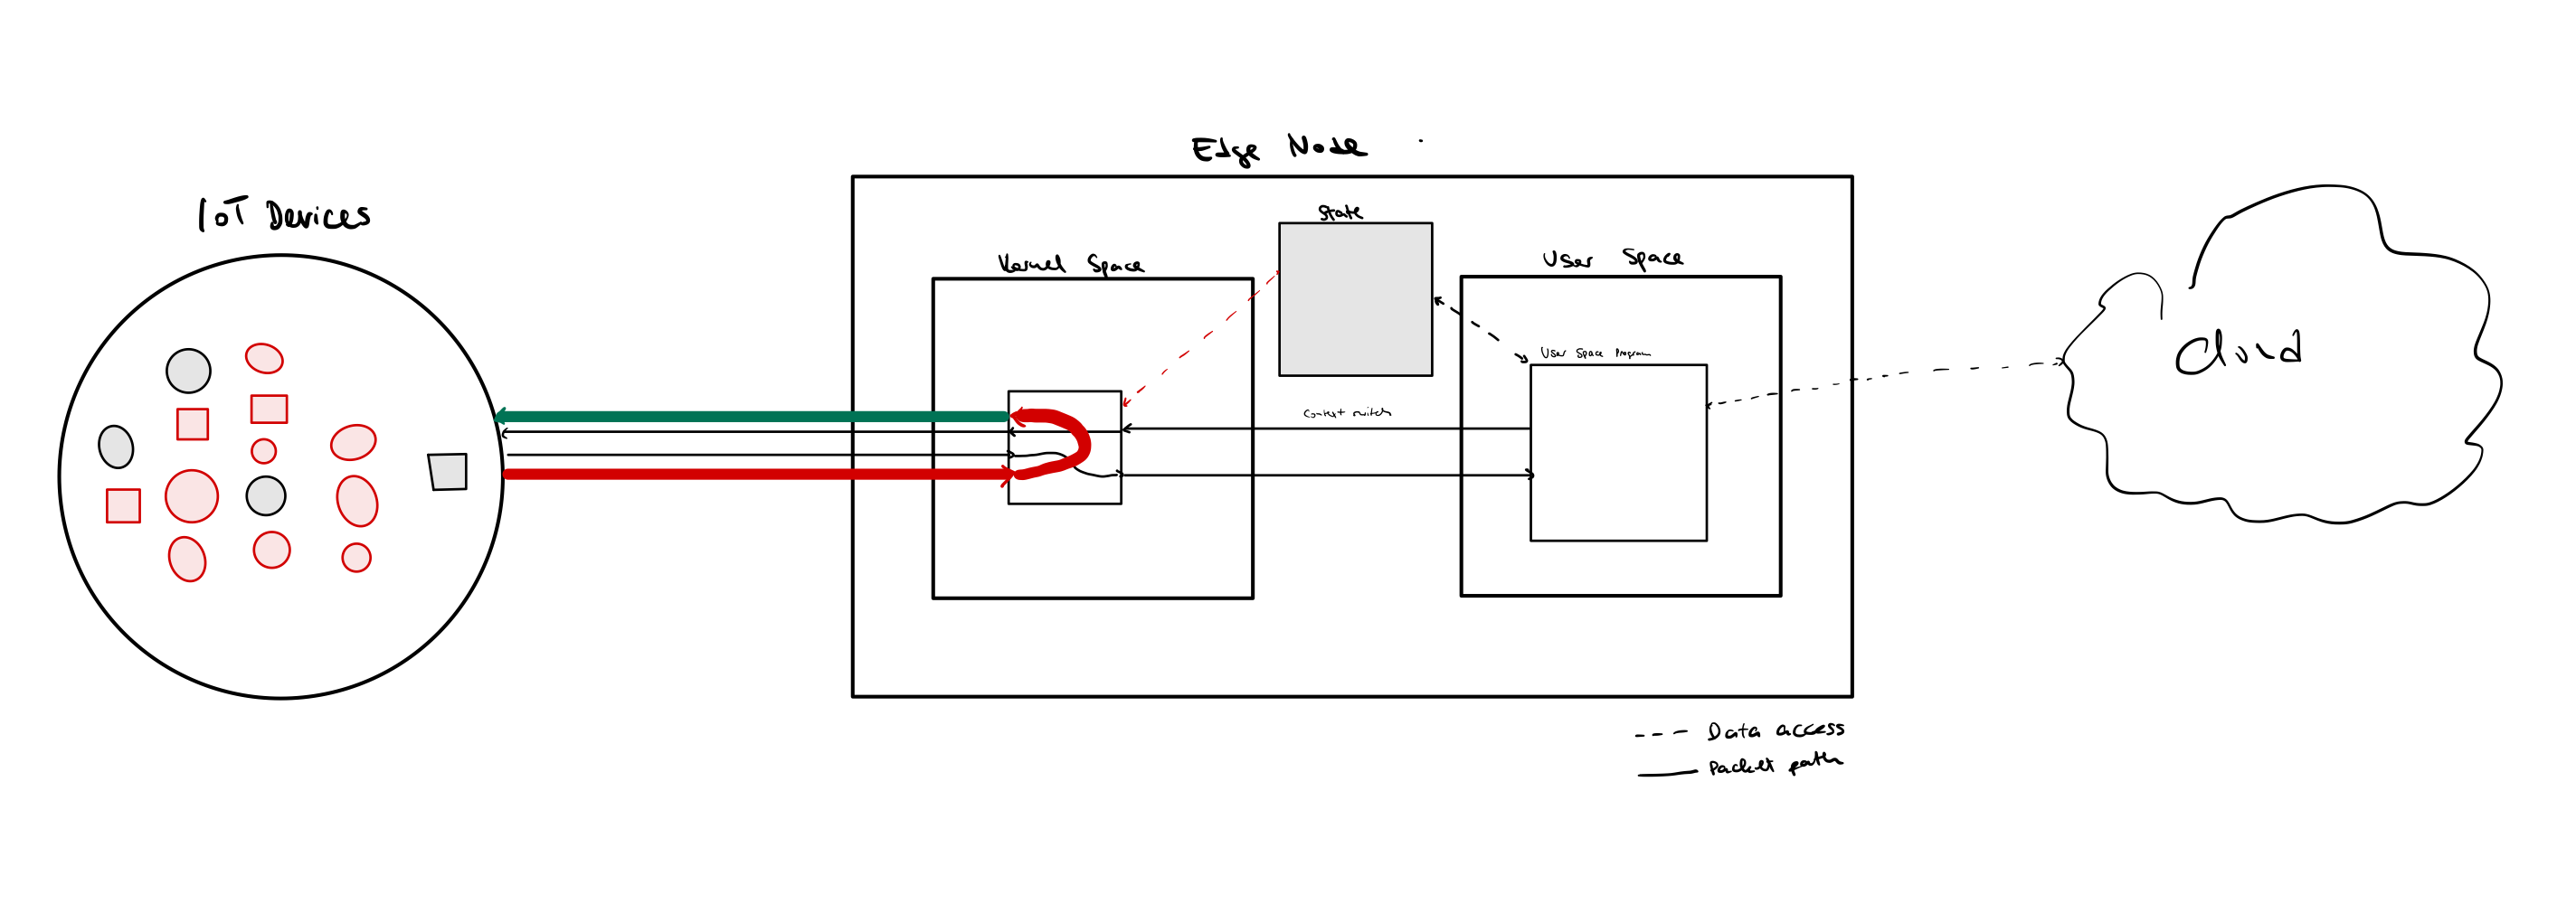
\includegraphics[width=\linewidth]{communication_after}
       \caption{communication after%
       \label{fig:communication_after}}%
\end{figure}
